% REV01 Wed 23 Jun 2021 06:07:34 WIB
% START Tue 04 May 2021 13:55:16 WIB

\chapter{IN WHICH AN INNOCENT ELOPEMENT OCCURS}

The minion of fortune and the worm of the hour, or in less cutting
language, Nicodemus Boffin, Esquire, the Golden Dustman, had become
as much at home in his eminently aristocratic family mansion as he
was likely ever to be. He could not but feel that, like an eminently
aristocratic family cheese, it was much too large for his wants, and
bred an infinite amount of parasites; but he was content to regard this
drawback on his property as a sort of perpetual Legacy Duty. He felt the
more resigned to it, forasmuch as Mrs Boffin enjoyed herself completely,
and Miss Bella was delighted.

That young lady was, no doubt, an acquisition to the Boffins. She
was far too pretty to be unattractive anywhere, and far too quick of
perception to be below the tone of her new career. Whether it improved
her heart might be a matter of taste that was open to question; but as
touching another matter of taste, its improvement of her appearance and
manner, there could be no question whatever.

And thus it soon came about that Miss Bella began to set Mrs Boffin
right; and even further, that Miss Bella began to feel ill at ease, and
as it were responsible, when she saw Mrs Boffin going wrong. Not that so
sweet a disposition and so sound a nature could ever go very wrong even
among the great visiting authorities who agreed that the Boffins were
‘charmingly vulgar’ (which for certain was not their own case in saying
so), but that when she made a slip on the social ice on which all the
children of Podsnappery, with genteel souls to be saved, are required to
skate in circles, or to slide in long rows, she inevitably tripped Miss
Bella up (so that young lady felt), and caused her to experience great
confusion under the glances of the more skilful performers engaged in
those ice-exercises.

At Miss Bella’s time of life it was not to be expected that she should
examine herself very closely on the congruity or stability of her
position in Mr Boffin’s house. And as she had never been sparing of
complaints of her old home when she had no other to compare it with,
so there was no novelty of ingratitude or disdain in her very much
preferring her new one.

‘An invaluable man is Rokesmith,’ said Mr Boffin, after some two or
three months. ‘But I can’t quite make him out.’

Neither could Bella, so she found the subject rather interesting.

‘He takes more care of my affairs, morning, noon, and night,’ said Mr
Boffin, ‘than fifty other men put together either could or would; and
yet he has ways of his own that are like tying a scaffolding-pole right
across the road, and bringing me up short when I am almost a-walking arm
in arm with him.’

‘May I ask how so, sir?’ inquired Bella.

‘Well, my dear,’ said Mr Boffin, ‘he won’t meet any company here, but
you. When we have visitors, I should wish him to have his regular place
at the table like ourselves; but no, he won’t take it.’

‘If he considers himself above it,’ said Miss Bella, with an airy toss
of her head, ‘I should leave him alone.’

‘It ain’t that, my dear,’ replied Mr Boffin, thinking it over. ‘He don’t
consider himself above it.’

‘Perhaps he considers himself beneath it,’ suggested Bella. ‘If so, he
ought to know best.’

‘No, my dear; nor it ain’t that, neither. No,’ repeated Mr Boffin, with
a shake of his head, after again thinking it over; ‘Rokesmith’s a modest
man, but he don’t consider himself beneath it.’

‘Then what does he consider, sir?’ asked Bella.

‘Dashed if I know!’ said Mr Boffin. ‘It seemed at first as if it
was only Lightwood that he objected to meet. And now it seems to be
everybody, except you.’

Oho! thought Miss Bella. ‘In--deed! That’s it, is it!’ For Mr Mortimer
Lightwood had dined there two or three times, and she had met him
elsewhere, and he had shown her some attention. ‘Rather cool in a
Secretary--and Pa’s lodger--to make me the subject of his jealousy!’

That Pa’s daughter should be so contemptuous of Pa’s lodger was odd;
but there were odder anomalies than that in the mind of the spoilt girl:
spoilt first by poverty, and then by wealth. Be it this history’s part,
however, to leave them to unravel themselves.

‘A little too much, I think,’ Miss Bella reflected scornfully, ‘to
have Pa’s lodger laying claim to me, and keeping eligible people off!
A little too much, indeed, to have the opportunities opened to me by Mr
and Mrs Boffin, appropriated by a mere Secretary and Pa’s lodger!’

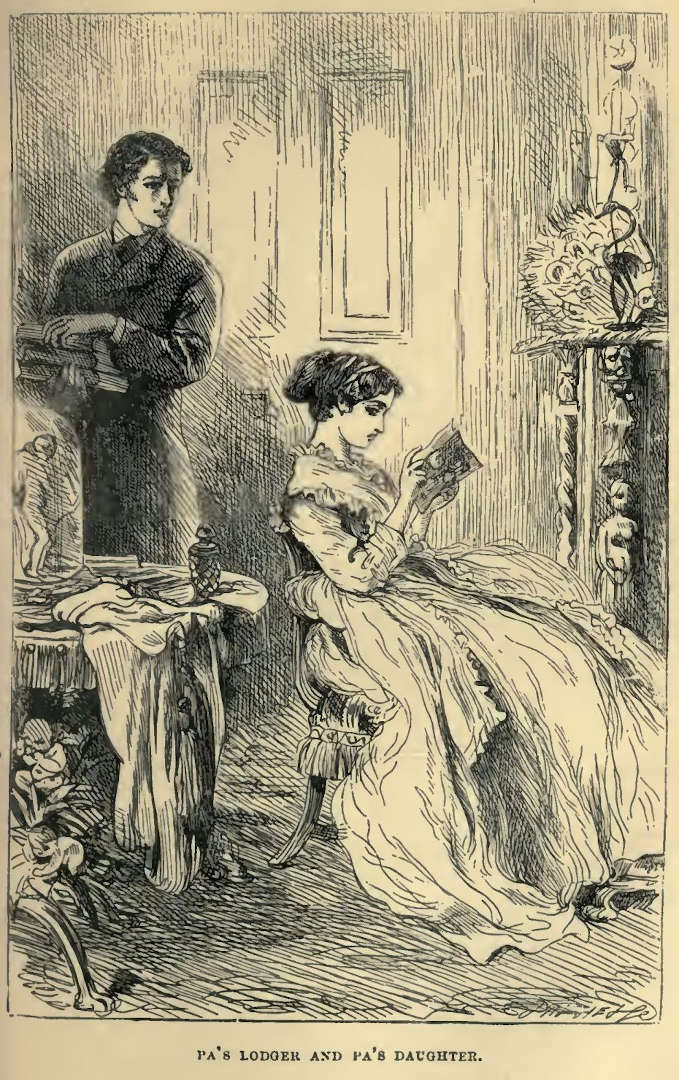
\includegraphics[scale=2.3]{02-08-01}

Yet it was not so very long ago that Bella had been fluttered by the
discovery that this same Secretary and lodger seem to like her. Ah! but
the eminently aristocratic mansion and Mrs Boffin’s dressmaker had not
come into play then.

In spite of his seemingly retiring manners a very intrusive person, this
Secretary and lodger, in Miss Bella’s opinion. Always a light in his
office-room when we came home from the play or Opera, and he always at
the carriage-door to hand us out. Always a provoking radiance too on
Mrs Boffin’s face, and an abominably cheerful reception of him, as if it
were possible seriously to approve what the man had in his mind!

‘You never charge me, Miss Wilfer,’ said the Secretary, encountering her
by chance alone in the great drawing-room, ‘with commissions for home.
I shall always be happy to execute any commands you may have in that
direction.’

‘Pray what may you mean, Mr Rokesmith?’ inquired Miss Bella, with
languidly drooping eyelids.

‘By home? I mean your father’s house at Holloway.’

She coloured under the retort--so skilfully thrust, that the words
seemed to be merely a plain answer, given in plain good faith--and said,
rather more emphatically and sharply:

‘What commissions and commands are you speaking of?’

‘Only little words of remembrance as I assume you sent somehow or
other,’ replied the Secretary with his former air. ‘It would be a
pleasure to me if you would make me the bearer of them. As you know, I
come and go between the two houses every day.’

‘You needn’t remind me of that, sir.’

She was too quick in this petulant sally against ‘Pa’s lodger’; and she
felt that she had been so when she met his quiet look.

‘They don’t send many--what was your expression?--words of remembrance
to me,’ said Bella, making haste to take refuge in ill-usage.

‘They frequently ask me about you, and I give them such slight
intelligence as I can.’

‘I hope it’s truly given,’ exclaimed Bella.

‘I hope you cannot doubt it, for it would be very much against you, if
you could.’

‘No, I do not doubt it. I deserve the reproach, which is very just
indeed. I beg your pardon, Mr Rokesmith.’

‘I should beg you not to do so, but that it shows you to such admirable
advantage,’ he replied with earnestness. ‘Forgive me; I could not help
saying that. To return to what I have digressed from, let me add that
perhaps they think I report them to you, deliver little messages, and
the like. But I forbear to trouble you, as you never ask me.’

‘I am going, sir,’ said Bella, looking at him as if he had reproved her,
‘to see them tomorrow.’

‘Is that,’ he asked, hesitating, ‘said to me, or to them?’

‘To which you please.’

‘To both? Shall I make it a message?’

‘You can if you like, Mr Rokesmith. Message or no message, I am going to
see them tomorrow.’

‘Then I will tell them so.’

He lingered a moment, as though to give her the opportunity of
prolonging the conversation if she wished. As she remained silent, he
left her. Two incidents of the little interview were felt by Miss Bella
herself, when alone again, to be very curious. The first was, that he
unquestionably left her with a penitent air upon her, and a penitent
feeling in her heart. The second was, that she had not an intention or
a thought of going home, until she had announced it to him as a settled
design.

‘What can I mean by it, or what can he mean by it?’ was her mental
inquiry: ‘He has no right to any power over me, and how do I come to
mind him when I don’t care for him?’

Mrs Boffin, insisting that Bella should make tomorrow’s expedition
in the chariot, she went home in great grandeur. Mrs Wilfer and Miss
Lavinia had speculated much on the probabilities and improbabilities of
her coming in this gorgeous state, and, on beholding the chariot from
the window at which they were secreted to look out for it, agreed
that it must be detained at the door as long as possible, for the
mortification and confusion of the neighbours. Then they repaired to
the usual family room, to receive Miss Bella with a becoming show of
indifference.

The family room looked very small and very mean, and the downward
staircase by which it was attained looked very narrow and very crooked.
The little house and all its arrangements were a poor contrast to the
eminently aristocratic dwelling. ‘I can hardly believe,’ thought Bella,
‘that I ever did endure life in this place!’

Gloomy majesty on the part of Mrs Wilfer, and native pertness on the
part of Lavvy, did not mend the matter. Bella really stood in natural
need of a little help, and she got none.

‘This,’ said Mrs Wilfer, presenting a cheek to be kissed, as sympathetic
and responsive as the back of the bowl of a spoon, ‘is quite an honour!
You will probably find your sister Lavvy grown, Bella.’

‘Ma,’ Miss Lavinia interposed, ‘there can be no objection to your being
aggravating, because Bella richly deserves it; but I really must request
that you will not drag in such ridiculous nonsense as my having grown
when I am past the growing age.’

‘I grew, myself,’ Mrs Wilfer sternly proclaimed, ‘after I was married.’

‘Very well, Ma,’ returned Lavvy, ‘then I think you had much better have
left it alone.’

The lofty glare with which the majestic woman received this answer,
might have embarrassed a less pert opponent, but it had no effect upon
Lavinia: who, leaving her parent to the enjoyment of any amount of
glaring at she might deem desirable under the circumstances, accosted
her sister, undismayed.

‘I suppose you won’t consider yourself quite disgraced, Bella, if I give
you a kiss? Well! And how do you do, Bella? And how are your Boffins?’

‘Peace!’ exclaimed Mrs Wilfer. ‘Hold! I will not suffer this tone of
levity.’

‘My goodness me! How are your Spoffins, then?’ said Lavvy, ‘since Ma so
very much objects to your Boffins.’

‘Impertinent girl! Minx!’ said Mrs Wilfer, with dread severity.

‘I don’t care whether I am a Minx, or a Sphinx,’ returned Lavinia,
coolly, tossing her head; ‘it’s exactly the same thing to me, and I’d
every bit as soon be one as the other; but I know this--I’ll not grow
after I’m married!’

‘You will not? YOU will not?’ repeated Mrs Wilfer, solemnly.

‘No, Ma, I will not. Nothing shall induce me.’

Mrs Wilfer, having waved her gloves, became loftily pathetic.

‘But it was to be expected;’ thus she spake. ‘A child of mine deserts me
for the proud and prosperous, and another child of mine despises me. It
is quite fitting.’

‘Ma,’ Bella struck in, ‘Mr and Mrs Boffin are prosperous, no doubt; but
you have no right to say they are proud. You must know very well that
they are not.’

‘In short, Ma,’ said Lavvy, bouncing over to the enemy without a word
of notice, ‘you must know very well--or if you don’t, more shame for
you!--that Mr and Mrs Boffin are just absolute perfection.’

‘Truly,’ returned Mrs Wilfer, courteously receiving the deserter, ‘it
would seem that we are required to think so. And this, Lavinia, is
my reason for objecting to a tone of levity. Mrs Boffin (of whose
physiognomy I can never speak with the composure I would desire to
preserve), and your mother, are not on terms of intimacy. It is not
for a moment to be supposed that she and her husband dare to presume to
speak of this family as the Wilfers. I cannot therefore condescend to
speak of them as the Boffins. No; for such a tone--call it familiarity,
levity, equality, or what you will--would imply those social
interchanges which do not exist. Do I render myself intelligible?’

Without taking the least notice of this inquiry, albeit delivered in an
imposing and forensic manner, Lavinia reminded her sister, ‘After all,
you know, Bella, you haven’t told us how your Whatshisnames are.’

‘I don’t want to speak of them here,’ replied Bella, suppressing
indignation, and tapping her foot on the floor. ‘They are much too kind
and too good to be drawn into these discussions.’

‘Why put it so?’ demanded Mrs Wilfer, with biting sarcasm. ‘Why adopt a
circuitous form of speech? It is polite and it is obliging; but why do
it? Why not openly say that they are much too kind and too good for US?
We understand the allusion. Why disguise the phrase?’

‘Ma,’ said Bella, with one beat of her foot, ‘you are enough to drive a
saint mad, and so is Lavvy.’

‘Unfortunate Lavvy!’ cried Mrs Wilfer, in a tone of commiseration. ‘She
always comes for it. My poor child!’ But Lavvy, with the suddenness of
her former desertion, now bounced over to the other enemy: very sharply
remarking, ‘Don’t patronize ME, Ma, because I can take care of myself.’

‘I only wonder,’ resumed Mrs Wilfer, directing her observations to her
elder daughter, as safer on the whole than her utterly unmanageable
younger, ‘that you found time and inclination to tear yourself from
Mr and Mrs Boffin, and come to see us at all. I only wonder that our
claims, contending against the superior claims of Mr and Mrs Boffin,
had any weight. I feel I ought to be thankful for gaining so much, in
competition with Mr and Mrs Boffin.’ (The good lady bitterly emphasized
the first letter of the word Boffin, as if it represented her chief
objection to the owners of that name, and as if she could have born
Doffin, Moffin, or Poffin much better.)

‘Ma,’ said Bella, angrily, ‘you force me to say that I am truly sorry I
did come home, and that I never will come home again, except when poor
dear Pa is here. For, Pa is too magnanimous to feel envy and spite
towards my generous friends, and Pa is delicate enough and gentle enough
to remember the sort of little claim they thought I had upon them and
the unusually trying position in which, through no act of my own, I had
been placed. And I always did love poor dear Pa better than all the rest
of you put together, and I always do and I always shall!’

Here Bella, deriving no comfort from her charming bonnet and her elegant
dress, burst into tears.

‘I think, R.W.,’ cried Mrs Wilfer, lifting up her eyes and
apostrophising the air, ‘that if you were present, it would be a
trial to your feelings to hear your wife and the mother of your family
depreciated in your name. But Fate has spared you this, R.W., whatever
it may have thought proper to inflict upon her!’

Here Mrs Wilfer burst into tears.

‘I hate the Boffins!’ protested Miss Lavinia. ‘I don’t care who objects
to their being called the Boffins. I WILL call ‘em the Boffins. The
Boffins, the Boffins, the Boffins! And I say they are mischief-making
Boffins, and I say the Boffins have set Bella against me, and I tell the
Boffins to their faces:’ which was not strictly the fact, but the
young lady was excited: ‘that they are detestable Boffins, disreputable
Boffins, odious Boffins, beastly Boffins. There!’

Here Miss Lavinia burst into tears.

The front garden-gate clanked, and the Secretary was seen coming at a
brisk pace up the steps. ‘Leave Me to open the door to him,’ said Mrs
Wilfer, rising with stately resignation as she shook her head and dried
her eyes; ‘we have at present no stipendiary girl to do so. We have
nothing to conceal. If he sees these traces of emotion on our cheeks,
let him construe them as he may.’

With those words she stalked out. In a few moments she stalked in again,
proclaiming in her heraldic manner, ‘Mr Rokesmith is the bearer of a
packet for Miss Bella Wilfer.’

Mr Rokesmith followed close upon his name, and of course saw what was
amiss. But he discreetly affected to see nothing, and addressed Miss
Bella.

‘Mr Boffin intended to have placed this in the carriage for you
this morning. He wished you to have it, as a little keepsake he had
prepared--it is only a purse, Miss Wilfer--but as he was disappointed in
his fancy, I volunteered to come after you with it.’

Bella took it in her hand, and thanked him.

‘We have been quarrelling here a little, Mr Rokesmith, but not more than
we used; you know our agreeable ways among ourselves. You find me just
going. Good-bye, mamma. Good-bye, Lavvy!’ and with a kiss for each Miss
Bella turned to the door. The Secretary would have attended her, but
Mrs Wilfer advancing and saying with dignity, ‘Pardon me! Permit me to
assert my natural right to escort my child to the equipage which is
in waiting for her,’ he begged pardon and gave place. It was a very
magnificent spectacle indeed, to see Mrs Wilfer throw open the
house-door, and loudly demand with extended gloves, ‘The male domestic
of Mrs Boffin!’ To whom presenting himself, she delivered the brief but
majestic charge, ‘Miss Wilfer. Coming out!’ and so delivered her over,
like a female Lieutenant of the Tower relinquishing a State Prisoner.
The effect of this ceremonial was for some quarter of an hour afterwards
perfectly paralyzing on the neighbours, and was much enhanced by the
worthy lady airing herself for that term in a kind of splendidly serene
trance on the top step.

When Bella was seated in the carriage, she opened the little packet in
her hand. It contained a pretty purse, and the purse contained a bank
note for fifty pounds. ‘This shall be a joyful surprise for poor dear
Pa,’ said Bella, ‘and I’ll take it myself into the City!’

As she was uninformed respecting the exact locality of the place of
business of Chicksey Veneering and Stobbles, but knew it to be near
Mincing Lane, she directed herself to be driven to the corner of that
darksome spot. Thence she despatched ‘the male domestic of Mrs Boffin,’
in search of the counting-house of Chicksey Veneering and Stobbles, with
a message importing that if R. Wilfer could come out, there was a lady
waiting who would be glad to speak with him. The delivery of these
mysterious words from the mouth of a footman caused so great an
excitement in the counting-house, that a youthful scout was instantly
appointed to follow Rumty, observe the lady, and come in with his
report. Nor was the agitation by any means diminished, when the scout
rushed back with the intelligence that the lady was ‘a slap-up gal in a
bang-up chariot.’

Rumty himself, with his pen behind his ear under his rusty hat, arrived
at the carriage-door in a breathless condition, and had been fairly
lugged into the vehicle by his cravat and embraced almost unto choking,
before he recognized his daughter. ‘My dear child!’ he then panted,
incoherently. ‘Good gracious me! What a lovely woman you are! I thought
you had been unkind and forgotten your mother and sister.’

‘I have just been to see them, Pa dear.’

‘Oh! and how--how did you find your mother?’ asked R. W., dubiously.

‘Very disagreeable, Pa, and so was Lavvy.’

‘They are sometimes a little liable to it,’ observed the patient cherub;
‘but I hope you made allowances, Bella, my dear?’

‘No. I was disagreeable too, Pa; we were all of us disagreeable
together. But I want you to come and dine with me somewhere, Pa.’

‘Why, my dear, I have already partaken of a--if one might mention such
an article in this superb chariot--of a--Saveloy,’ replied R. Wilfer,
modestly dropping his voice on the word, as he eyed the canary-coloured
fittings.

‘Oh! That’s nothing, Pa!’

‘Truly, it ain’t as much as one could sometimes wish it to be, my
dear,’ he admitted, drawing his hand across his mouth. ‘Still, when
circumstances over which you have no control, interpose obstacles
between yourself and Small Germans, you can’t do better than bring a
contented mind to hear on’--again dropping his voice in deference to the
chariot--‘Saveloys!’

‘You poor good Pa! Pa, do, I beg and pray, get leave for the rest of the
day, and come and pass it with me!’

‘Well, my dear, I’ll cut back and ask for leave.’

‘But before you cut back,’ said Bella, who had already taken him by the
chin, pulled his hat off, and begun to stick up his hair in her old way,
‘do say that you are sure I am giddy and inconsiderate, but have never
really slighted you, Pa.’

‘My dear, I say it with all my heart. And might I likewise observe,’ her
father delicately hinted, with a glance out at window, ‘that perhaps
it might be calculated to attract attention, having one’s hair publicly
done by a lovely woman in an elegant turn-out in Fenchurch Street?’

Bella laughed and put on his hat again. But when his boyish figure
bobbed away, its shabbiness and cheerful patience smote the tears out
of her eyes. ‘I hate that Secretary for thinking it of me,’ she said to
herself, ‘and yet it seems half true!’

Back came her father, more like a boy than ever, in his release from
school. ‘All right, my dear. Leave given at once. Really very handsomely
done!’

‘Now where can we find some quiet place, Pa, in which I can wait for you
while you go on an errand for me, if I send the carriage away?’

It demanded cogitation. ‘You see, my dear,’ he explained, ‘you really
have become such a very lovely woman, that it ought to be a very quiet
place.’ At length he suggested, ‘Near the garden up by the Trinity House
on Tower Hill.’ So, they were driven there, and Bella dismissed the
chariot; sending a pencilled note by it to Mrs Boffin, that she was with
her father.

‘Now, Pa, attend to what I am going to say, and promise and vow to be
obedient.’

‘I promise and vow, my dear.’

‘You ask no questions. You take this purse; you go to the nearest place
where they keep everything of the very very best, ready made; you buy
and put on, the most beautiful suit of clothes, the most beautiful hat,
and the most beautiful pair of bright boots (patent leather, Pa, mind!)
that are to be got for money; and you come back to me.’

‘But, my dear Bella--’

‘Take care, Pa!’ pointing her forefinger at him, merrily. ‘You have
promised and vowed. It’s perjury, you know.’

There was water in the foolish little fellow’s eyes, but she kissed them
dry (though her own were wet), and he bobbed away again. After half an
hour, he came back, so brilliantly transformed, that Bella was obliged
to walk round him in ecstatic admiration twenty times, before she could
draw her arm through his, and delightedly squeeze it.

‘Now, Pa,’ said Bella, hugging him close, ‘take this lovely woman out to
dinner.’

‘Where shall we go, my dear?’

‘Greenwich!’ said Bella, valiantly. ‘And be sure you treat this lovely
woman with everything of the best.’

While they were going along to take boat, ‘Don’t you wish, my dear,’
said R. W., timidly, ‘that your mother was here?’

‘No, I don’t, Pa, for I like to have you all to myself to-day. I was
always your little favourite at home, and you were always mine. We have
run away together often, before now; haven’t we, Pa?’

‘Ah, to be sure we have! Many a Sunday when your mother was--was a
little liable to it,’ repeating his former delicate expression after
pausing to cough.

‘Yes, and I am afraid I was seldom or never as good as I ought to have
been, Pa. I made you carry me, over and over again, when you should
have made me walk; and I often drove you in harness, when you would much
rather have sat down and read your news-paper: didn’t I?’

‘Sometimes, sometimes. But Lor, what a child you were! What a companion
you were!’

‘Companion? That’s just what I want to be to-day, Pa.’

‘You are safe to succeed, my love. Your brothers and sisters have all
in their turns been companions to me, to a certain extent, but only to a
certain extent. Your mother has, throughout life, been a companion that
any man might--might look up to--and--and commit the sayings of, to
memory--and--form himself upon--if he--’

‘If he liked the model?’ suggested Bella.

‘We-ell, ye-es,’ he returned, thinking about it, not quite satisfied
with the phrase: ‘or perhaps I might say, if it was in him. Supposing,
for instance, that a man wanted to be always marching, he would find
your mother an inestimable companion. But if he had any taste for
walking, or should wish at any time to break into a trot, he might
sometimes find it a little difficult to keep step with your mother.
Or take it this way, Bella,’ he added, after a moment’s reflection;
‘Supposing that a man had to go through life, we won’t say with a
companion, but we’ll say to a tune. Very good. Supposing that the tune
allotted to him was the Dead March in Saul. Well. It would be a very
suitable tune for particular occasions--none better--but it would
be difficult to keep time with in the ordinary run of domestic
transactions. For instance, if he took his supper after a hard day, to
the Dead March in Saul, his food might be likely to sit heavy on him.
Or, if he was at any time inclined to relieve his mind by singing a
comic song or dancing a hornpipe, and was obliged to do it to the Dead
March in Saul, he might find himself put out in the execution of his
lively intentions.’

‘Poor Pa!’ thought Bella, as she hung upon his arm.

‘Now, what I will say for you, my dear,’ the cherub pursued mildly and
without a notion of complaining, ‘is, that you are so adaptable. So
adaptable.’

‘Indeed I am afraid I have shown a wretched temper, Pa. I am afraid
I have been very complaining, and very capricious. I seldom or never
thought of it before. But when I sat in the carriage just now and saw
you coming along the pavement, I reproached myself.’

‘Not at all, my dear. Don’t speak of such a thing.’

A happy and a chatty man was Pa in his new clothes that day. Take it
for all in all, it was perhaps the happiest day he had ever known in his
life; not even excepting that on which his heroic partner had approached
the nuptial altar to the tune of the Dead March in Saul.

The little expedition down the river was delightful, and the little
room overlooking the river into which they were shown for dinner was
delightful. Everything was delightful. The park was delightful, the
punch was delightful, the dishes of fish were delightful, the wine
was delightful. Bella was more delightful than any other item in the
festival; drawing Pa out in the gayest manner; making a point of always
mentioning herself as the lovely woman; stimulating Pa to order things,
by declaring that the lovely woman insisted on being treated with them;
and in short causing Pa to be quite enraptured with the consideration
that he WAS the Pa of such a charming daughter.

And then, as they sat looking at the ships and steamboats making their
way to the sea with the tide that was running down, the lovely woman
imagined all sorts of voyages for herself and Pa. Now, Pa, in the
character of owner of a lumbering square-sailed collier, was tacking
away to Newcastle, to fetch black diamonds to make his fortune with;
now, Pa was going to China in that handsome threemasted ship, to bring
home opium, with which he would for ever cut out Chicksey Veneering
and Stobbles, and to bring home silks and shawls without end for the
decoration of his charming daughter. Now, John Harmon’s disastrous fate
was all a dream, and he had come home and found the lovely woman just
the article for him, and the lovely woman had found him just the article
for her, and they were going away on a trip, in their gallant bark,
to look after their vines, with streamers flying at all points, a band
playing on deck and Pa established in the great cabin. Now, John Harmon
was consigned to his grave again, and a merchant of immense wealth
(name unknown) had courted and married the lovely woman, and he was
so enormously rich that everything you saw upon the river sailing or
steaming belonged to him, and he kept a perfect fleet of yachts for
pleasure, and that little impudent yacht which you saw over there, with
the great white sail, was called The Bella, in honour of his wife, and
she held her state aboard when it pleased her, like a modern Cleopatra.
Anon, there would embark in that troop-ship when she got to Gravesend, a
mighty general, of large property (name also unknown), who wouldn’t
hear of going to victory without his wife, and whose wife was the lovely
woman, and she was destined to become the idol of all the red coats and
blue jackets alow and aloft. And then again: you saw that ship being
towed out by a steam-tug? Well! where did you suppose she was going to?
She was going among the coral reefs and cocoa-nuts and all that sort of
thing, and she was chartered for a fortunate individual of the name
of Pa (himself on board, and much respected by all hands), and she
was going, for his sole profit and advantage, to fetch a cargo of
sweet-smelling woods, the most beautiful that ever were seen, and the
most profitable that ever were heard of; and her cargo would be a great
fortune, as indeed it ought to be: the lovely woman who had purchased
her and fitted her expressly for this voyage, being married to an Indian
Prince, who was a Something-or-Other, and who wore Cashmere shawls all
over himself and diamonds and emeralds blazing in his turban, and was
beautifully coffee-coloured and excessively devoted, though a little too
jealous. Thus Bella ran on merrily, in a manner perfectly enchanting to
Pa, who was as willing to put his head into the Sultan’s tub of water as
the beggar-boys below the window were to put THEIR heads in the mud.

‘I suppose, my dear,’ said Pa after dinner, ‘we may come to the
conclusion at home, that we have lost you for good?’

Bella shook her head. Didn’t know. Couldn’t say. All she was able to
report was, that she was most handsomely supplied with everything she
could possibly want, and that whenever she hinted at leaving Mr and Mrs
Boffin, they wouldn’t hear of it.

‘And now, Pa,’ pursued Bella, ‘I’ll make a confession to you. I am the
most mercenary little wretch that ever lived in the world.’

‘I should hardly have thought it of you, my dear,’ returned her father,
first glancing at himself; and then at the dessert.

‘I understand what you mean, Pa, but it’s not that. It’s not that I care
for money to keep as money, but I do care so much for what it will buy!’

‘Really I think most of us do,’ returned R. W.

‘But not to the dreadful extent that I do, Pa. O-o!’ cried Bella,
screwing the exclamation out of herself with a twist of her dimpled
chin. ‘I AM so mercenary!’

With a wistful glance R. W. said, in default of having anything better
to say: ‘About when did you begin to feel it coming on, my dear?’

‘That’s it, Pa. That’s the terrible part of it. When I was at home, and
only knew what it was to be poor, I grumbled but didn’t so much mind.
When I was at home expecting to be rich, I thought vaguely of all the
great things I would do. But when I had been disappointed of my splendid
fortune, and came to see it from day to day in other hands, and to have
before my eyes what it could really do, then I became the mercenary
little wretch I am.’

‘It’s your fancy, my dear.’

‘I can assure you it’s nothing of the sort, Pa!’ said Bella, nodding at
him, with her very pretty eyebrows raised as high as they would go, and
looking comically frightened. ‘It’s a fact. I am always avariciously
scheming.’

‘Lor! But how?’

‘I’ll tell you, Pa. I don’t mind telling YOU, because we have always
been favourites of each other’s, and because you are not like a Pa, but
more like a sort of a younger brother with a dear venerable chubbiness
on him. And besides,’ added Bella, laughing as she pointed a rallying
finger at his face, ‘because I have got you in my power. This is a
secret expedition. If ever you tell of me, I’ll tell of you. I’ll tell
Ma that you dined at Greenwich.’

‘Well; seriously, my dear,’ observed R. W., with some trepidation of
manner, ‘it might be as well not to mention it.’

‘Aha!’ laughed Bella. ‘I knew you wouldn’t like it, sir! So you keep my
confidence, and I’ll keep yours. But betray the lovely woman, and you
shall find her a serpent. Now, you may give me a kiss, Pa, and I should
like to give your hair a turn, because it has been dreadfully neglected
in my absence.’

R. W. submitted his head to the operator, and the operator went on
talking; at the same time putting separate locks of his hair through
a curious process of being smartly rolled over her two revolving
forefingers, which were then suddenly pulled out of it in opposite
lateral directions. On each of these occasions the patient winced and
winked.

‘I have made up my mind that I must have money, Pa. I feel that I can’t
beg it, borrow it, or steal it; and so I have resolved that I must marry
it.’

R. W. cast up his eyes towards her, as well as he could under the
operating circumstances, and said in a tone of remonstrance, ‘My de-ar
Bella!’

‘Have resolved, I say, Pa, that to get money I must marry money. In
consequence of which, I am always looking out for money to captivate.’

‘My de-a-r Bella!’

‘Yes, Pa, that is the state of the case. If ever there was a mercenary
plotter whose thoughts and designs were always in her mean occupation, I
am the amiable creature. But I don’t care. I hate and detest being
poor, and I won’t be poor if I can marry money. Now you are deliciously
fluffy, Pa, and in a state to astonish the waiter and pay the bill.’

‘But, my dear Bella, this is quite alarming at your age.’

‘I told you so, Pa, but you wouldn’t believe it,’ returned Bella, with a
pleasant childish gravity. ‘Isn’t it shocking?’

‘It would be quite so, if you fully knew what you said, my dear, or
meant it.’

‘Well, Pa, I can only tell you that I mean nothing else. Talk to me of
love!’ said Bella, contemptuously: though her face and figure certainly
rendered the subject no incongruous one. ‘Talk to me of fiery dragons!
But talk to me of poverty and wealth, and there indeed we touch upon
realities.’

‘My De-ar, this is becoming Awful--’ her father was emphatically
beginning: when she stopped him.

‘Pa, tell me. Did you marry money?’

‘You know I didn’t, my dear.’

Bella hummed the Dead March in Saul, and said, after all it signified
very little! But seeing him look grave and downcast, she took him round
the neck and kissed him back to cheerfulness again.

‘I didn’t mean that last touch, Pa; it was only said in joke. Now mind!
You are not to tell of me, and I’ll not tell of you. And more than that;
I promise to have no secrets from you, Pa, and you may make certain
that, whatever mercenary things go on, I shall always tell you all about
them in strict confidence.’

Fain to be satisfied with this concession from the lovely woman, R. W.
rang the bell, and paid the bill. ‘Now, all the rest of this, Pa,’ said
Bella, rolling up the purse when they were alone again, hammering it
small with her little fist on the table, and cramming it into one of the
pockets of his new waistcoat, ‘is for you, to buy presents with for them
at home, and to pay bills with, and to divide as you like, and spend
exactly as you think proper. Last of all take notice, Pa, that it’s
not the fruit of any avaricious scheme. Perhaps if it was, your little
mercenary wretch of a daughter wouldn’t make so free with it!’

After which, she tugged at his coat with both hands, and pulled him all
askew in buttoning that garment over the precious waistcoat pocket, and
then tied her dimples into her bonnet-strings in a very knowing way, and
took him back to London. Arrived at Mr Boffin’s door, she set him with
his back against it, tenderly took him by the ears as convenient handles
for her purpose, and kissed him until he knocked muffled double knocks
at the door with the back of his head. That done, she once more reminded
him of their compact and gaily parted from him.

Not so gaily, however, but that tears filled her eyes as he went away
down the dark street. Not so gaily, but that she several times said,
‘Ah, poor little Pa! Ah, poor dear struggling shabby little Pa!’
before she took heart to knock at the door. Not so gaily, but that the
brilliant furniture seemed to stare her out of countenance as if it
insisted on being compared with the dingy furniture at home. Not so
gaily, but that she fell into very low spirits sitting late in her own
room, and very heartily wept, as she wished, now that the deceased old
John Harmon had never made a will about her, now that the deceased young
John Harmon had lived to marry her. ‘Contradictory things to wish,’ said
Bella, ‘but my life and fortunes are so contradictory altogether that
what can I expect myself to be!’



